\documentclass{article}
% translate with >> pdflatex -shell-escape <file>

% This file is an extract of the PGFPLOTS manual, copyright by Christian Feuersaenger.
% 
% Feel free to use it as long as you cite the pgfplots manual properly.
%
% See
%   http://pgfplots.sourceforge.net/pgfplots.pdf
% for the complete manual.
%
% Any required input files (for <plot table> or <plot file> or the table package) can be downloaded
% at
% http://www.ctan.org/tex-archive/graphics/pgf/contrib/pgfplots/doc/latex/
% and
% http://www.ctan.org/tex-archive/graphics/pgf/contrib/pgfplots/doc/latex/plotdata/

\usepackage{pgfplots}
\pgfplotsset{compat=newest}

\pagestyle{empty}
\usepgfplotslibrary{patchplots}

\begin{document}
% requires \usepgfplotslibrary{patchplots}
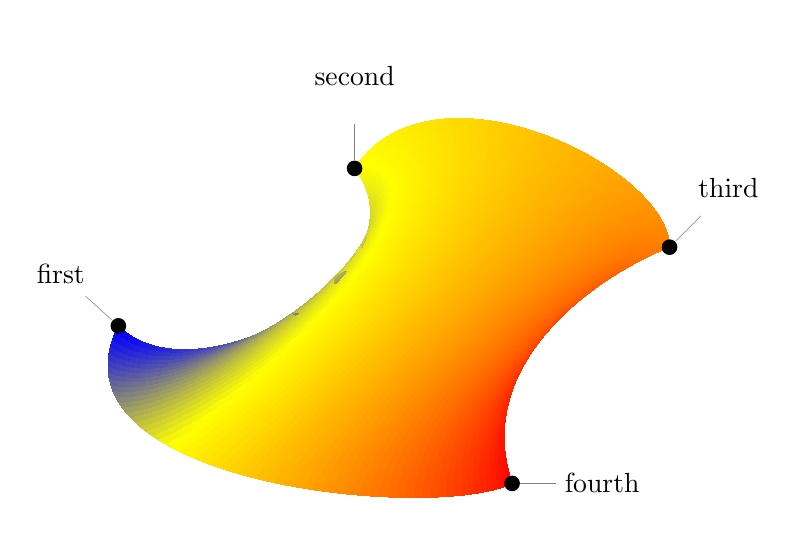
\begin{tikzpicture}
\begin{axis}[
	% tell pgfplots to "grab" the axis at its internal (0,0) coord:
    anchor=origin,      
	% tell pgfplots to place its anchor at (0,0):
	% (This is actually the default and can be omitted)
    at={(0pt,0pt)},
	% tell pgfplots to use the "natural" dimensions:
    disabledatascaling,
	% tell pgfplots to use the same unit vectors as tikz:
    x=1cm,y=1cm,
	%
	hide axis,
]
\addplot[patch,patch type=coons,
	shader=interp,point meta=explicit] 
coordinates {
	(0,0)   [0] % first corner
	(1,-1)  [0] % bezier control point between (0) and (3)
	(4,0.7) [0] % bezier control point between (0) and (3)
	%
	(3,2)   [1] % second corner
	(4,3.5) [1] % bezier control point between (3) and (6)
	(7,2)   [1] % bezier control point between (3) and (6)
	%
	(7,1)      [2] % third corner
	(6,0.6)    [2] % bezier control point between (6) and (9)
	(4.5,-0.5) [2] % bezier control point between (6) and (9)
	%
	(5,-2)   [3] % fourth corner
	(4,-2.5) [3] % bezier control point between (9) and (0)
	(-1,-2)  [3] % bezier control point between (9) and (0)
};
\end{axis}

% this requires pgf 2.10 
\begin{scope}[every node/.style={circle,inner sep=2pt,fill=black}]
\node[pin=140:first] at (0,0) {};
\node[pin=second]    at (3,2) {};
\node[pin=45:third]  at (7,1) {};
\node[pin=0:fourth]  at (5,-2) {};
\end{scope}
\end{tikzpicture}
\end{document}
